\section{Literature Review}
\label{sec:literaturereview}

\begin{figure}[h!]
  \centering
  \begin{subfigure}[b]{0.6\textwidth}
    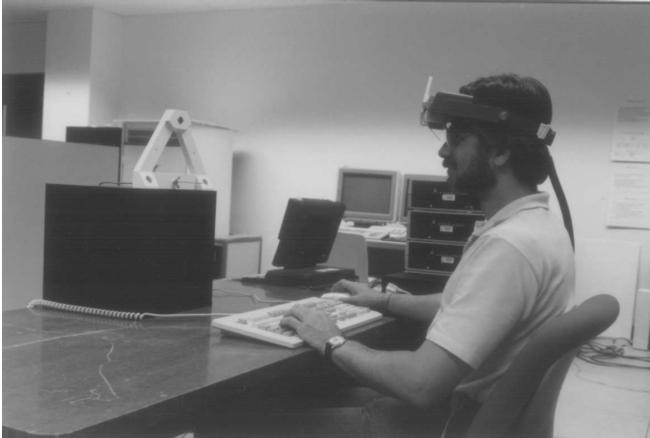
\includegraphics[width=\linewidth]{fig01.png}
    \caption{Feiner's window system with an HWD in 1993. The large black cube and white triangle are the transmitters for two 3D tracking systems. Tracker receivers on the head-mounted display, waist, and wrist.}
  \end{subfigure}
  \begin{subfigure}[b]{0.6\textwidth}
    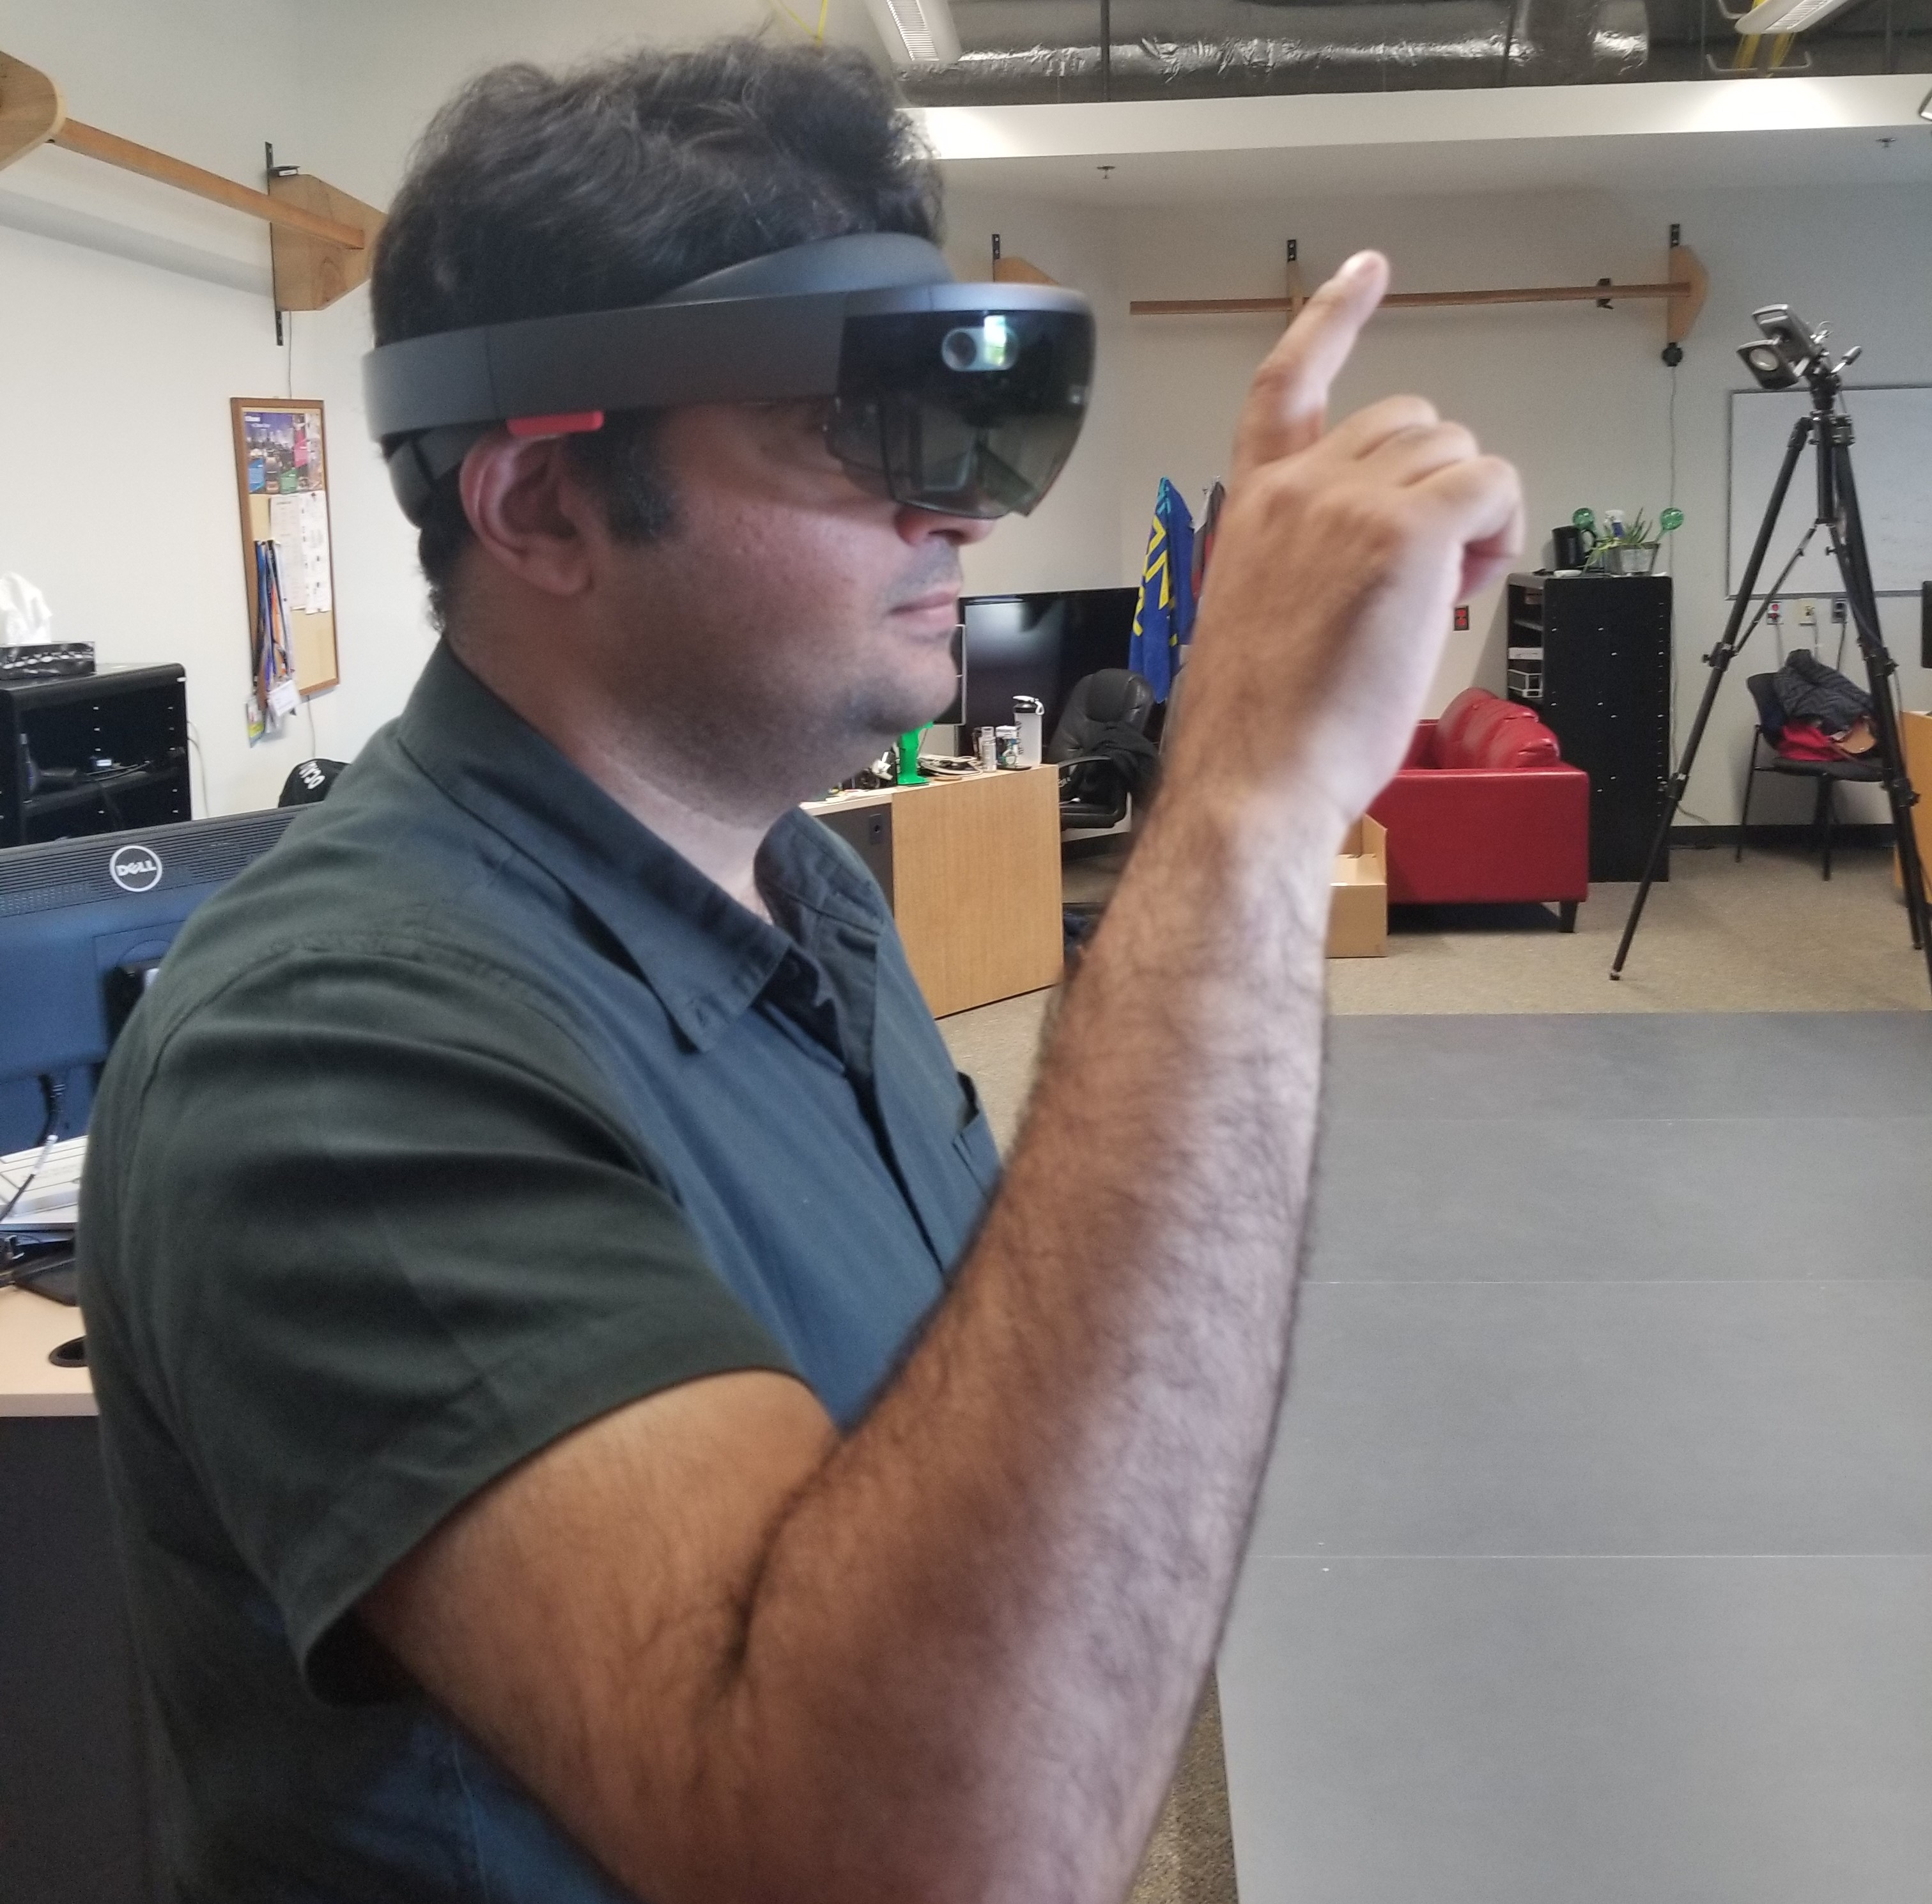
\includegraphics[width=\linewidth]{fig02.jpg}
    \caption{One of the latest ARHWDs released. It requires no external component and all the sensors are implemented with the device.}
  \end{subfigure}
  \caption{A Comparison of ARHWDs}
  \label{fig:compareARHWD}
\end{figure}
Augmented reality systems (AR) are defined as systems that enable real time interactions with virtual and real objects that coexist in the same space \cite{Azuma1997}. These systems come in many different forms such as head-worn displays, projections, and mobile devices that allow you to view virtual objects in the real world. For decades, researchers have observed the great potential of using augmented reality to enhance certain aspects in fields such as education and health. \cite{Bower2014} highlight the usage of mobile phones and tablets to overlay media onto the real world in order to make information available to students when they need it, on the spot. Bower et al. discuss the potential reduction of cognitive overload by providing students real time information. Augmented reality has also found a home within the health field, specifically the medical field, where it is used in various medical tasks and procedures.

In recent years, researchers have investigated the use of AR in order to improve surgical navigation. Both \cite{Okamoto2015} and \cite{Chen2015} developed AR-based simulations with the aim to improve the safety and reliability of surgery. Okamoto et al. developed an application for navigation surgery in the abdominal field. Their system leverage a see through display and a rigid scope that enables the surgeons to obtain a 3D view. Through their study, they are able to identify several problems such as organ deformity, evaluation of utility, portability and cost. In the same year, Chen et al. leveraged a head-worn display and created an application that was tested against actual patient structure data in a real world scenario. They verified and demonstrated the accuracy of their application was sufficient to meet clinical requirements. However, this is so far only true with a simulated environment. 

\cite{Barsom2016} details the effectiveness of augmented reality applications in medical training. These applications are used to blend virtual and digital elements with a physical environment in order to introduce new educational opportunities for medical professionals. Barsom et al. review seven applications over twenty-six studies and concluded that although these promising applications are generating public as well as scientific interest, they are lacking evidence in the literature that the applications are able to transfer information to the user.

This work will primarily be focused on head-worn see-through display such as the Microsoft Hololens \cite{Hololens}, a new headset that enables users to interact with virtual objects in the real world. Due to the novelty of this display and the ongoing development of the software required to create applications for this display, there are not many studies involving the Hololens as of yet. This however, has not stopped researchers in studying the design concepts of interactions with augmented displays. 

Designing interactions in AR has been a topic of discussion for as long as the concept of AR existed. In 1993, \cite{Feiner1993} looked into implementing 2D windows in a 3D augmented reality. This was one of the earliest works in augmented reality, and they were able to create a system that overlaid images on a see through display, simulating virtual windows containing information in a real-world environment (See figure \ref{fig:compareARHWD}). 

In a survey done by \cite{Azuma1997} to provide a beginning point for researchers interested in this area, outlined the advancements in 1997, the applications of AR, and some issues such as real-time tracking and portability. Many issues outlined by Azuma in his survey have been address in recent years. The hardware is only one part of the design required to create a smooth augmented experience. Future research focuses more on the interface and interactions with the virtual objects in the real world environment.

Early works, such as \cite{Bell2001} describe maintaining visual constraints on the virtual objects projected on the view plane. Simply put, they attempted to design an algorithm to aid in managing constraints such as locating related virtual objects or preventing the objects from occluding each other. Their algorithm yielded comfortable interactions, however, Bell et al. believed it could have been significantly improved. 

In subsequent years, a plethora of research on AR becomes a cycle and blend of outlining potentials, addressing issues at the time, and a survey of the state of AR. Works such as \cite{Zhong2003} and \cite{Boulanger2004} outline the potential in using AR in industrial training. \cite{Bower2014} look into the applications in education and its potential to improve learning in schools. In the health industry, researchers such as \cite{Barsom2016, Chan2017, Chen2015, Okamoto2015} look at AR's potential in surgery and medical training. However, many of the works outlining potentials do not develop as well as evaluate the application leading to inconclusive results.

Although in the past, there have seen very few works involving the use of augmented reality head-worn displays (ARHWDs), the popularity of the concept due to it's portability has been steadily increasing.Although, work such as The Personal Cockpit \cite{Ens2014}, an evaluated design space for effective task switching on ARHWDs and Ethreal Planes \cite{Ens2014a}, an extensively reviewed design framework provide guidelines to assist in the creation of meaningful layouts and interfaces to experiment with. As far as I know, there has not been any work done on determining the efficiency of using AR head-worn displays such as the Hololens to act as an aid in completing procedural or analytical tasks. 

